
\part{ImageJ User Interface\label{par:User-Interface1}}

Unlike most image processing programs ImageJ does not have a main
work area\nomenclature{GUI}{Graphical User Interface}. ImageJ's main
window is actually quite parsimonious containing only a menu bar (at
the top of the screen on the Mac) containing all the \nameref{par:Commands},
a \nameref{sub:Toolbar}, a \nameref{sub:Status-bar} and a \nameref{sub:Progress-bar}.
Images, histograms, profiles, widgets, etc.\ are displayed in additional
windows. Measurement results are displayed in the \nameref{sec:Results-Table}.
Most windows can be dragged around the screen and resized. 

\begin{figure}[h]
\noindent \begin{centering}
\caption[Main ImageJ window]{\textbf{\label{fig:The-ImageJ-window}The ImageJ window (version\,1.46j).}}
\vspace*{2pt}

\par\end{centering}

\noindent \begin{centering}
\setlength{\tabcolsep}{0pt}%
\begin{tabular}{>{\centering}p{6.45mm}>{\centering}p{6.45mm}>{\centering}p{6.45mm}>{\centering}p{6.45mm}>{\centering}p{6.45mm}>{\centering}p{6.45mm}>{\centering}p{6.45mm}>{\centering}p{6.45mm}>{\centering}p{6.45mm}>{\centering}p{6.45mm}>{\centering}p{6.45mm}>{\centering}p{6.45mm}>{\centering}p{6.45mm}>{\centering}p{6.45mm}>{\centering}p{6.45mm}>{\centering}p{6.45mm}>{\centering}p{6.45mm}>{\centering}p{6.45mm}>{\centering}p{6.45mm}>{\centering}p{6.45mm}>{\centering}p{6.45mm}}
{\small 1} & {\small 2} & {\small 3} & {\small 4} & {\small 5} & {\small 6} & {\small 7} & {\small 8} & {\small 9} & {\small 10} & {\small 11} & {\small 12} & {\small A} & {\small B} & {\small C} & {\small D} & {\small E} & {\small F} & {\small G} & {\small H} & {\small 13}\tabularnewline
\multicolumn{21}{c}{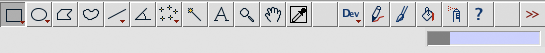
\includegraphics[width=136mm]{images/IJ_Window}}\tabularnewline
\noalign{\vskip-4.5pt}
\multicolumn{10}{l}{{\small \hspace*{15pt}\nameref{sub:Status-bar}}} & \multicolumn{11}{r}{{\small \nameref{sub:Progress-bar}\hspace*{15pt}}}\tabularnewline
\end{tabular}
\par\end{centering}

\noindent \begin{centering}
\vspace*{8pt}

\par\end{centering}

\noindent \centering{}\setlength{\tabcolsep}{0pt}~%
\begin{tabular}{>{\raggedright}m{6mm}>{\raggedright}p{72.5mm}>{\raggedright}p{9mm}>{\raggedright}p{49mm}}
{\small 1} & \multirow{2}{72.5mm}{{\small \nameref{sub:Rectangular-Selection-Tool} and \nameref{sub:Round-Rectangular-Selection}}} & {\small 8} & {\small \nameref{sub:Wand-Tool}}\tabularnewline
 &  & {\small 9} & {\small \nameref{sec:Text-Tool}}\tabularnewline
\noalign{\vskip\doublerulesep}
{\small 2} & \multirow{2}{72.5mm}{{\small \nameref{sub:Oval-Selection-Tool}, \nameref{sub:Elliptical-Selection-Tool}
and \nameref{sub:Brush-Selection-Tool} }} & {\small 10} & {\small \nameref{sec:Magnifying-Glass}}\tabularnewline
 &  & {\small 11} & {\small \nameref{sec:Scrolling-Tool}}\tabularnewline
\noalign{\vskip\doublerulesep}
{\small 3} & {\small \nameref{sub:Polygon-Selection-Tool}} & {\small 12} & {\small \nameref{sec:Color-Picker}}\tabularnewline
\noalign{\vskip\doublerulesep}
{\small 4} & {\small \nameref{sub:Freehand-Selection-Tool}} & {\small 13} & {\small \nameref{sec:ToolSwitcher}}\tabularnewline
\noalign{\vskip\doublerulesep}
{\small 5} & {\small \nameref{sub:Straight-Line-Selection}, \nameref{sub:Segmented-Line-Selection},
\nameref{sub:Freehand-Selection-Tool} and \nameref{sec:Arrow-Tool} } & {\small A--H} & \multirow{3}{49mm}{Customized tools installed from \filenameref{StartupMacros.txt},
\dirnameref{macros/toolsets/}, \dirnameref{macros/tools/} or \dirnameref{plugins/Tools/} }\tabularnewline
\noalign{\vskip\doublerulesep}
{\small 6} & {\small \nameref{sec:Angle-Tool}} &  & \tabularnewline
\noalign{\vskip\doublerulesep}
{\small 7} & {\small \nameref{sec:Point-Tool} and \nameref{sec:Multi-point-Tool}} &  & \tabularnewline
\end{tabular}
\end{figure}



\subsection*{Toolbar\label{sub:Toolbar}}

The ImageJ toolbar contains tools for making selections, drawings,
zooming and scrolling, etc. In addition, the right-side of the toolbar
contains seven slots that can host any of the \href{http://imagej.nih.gov/ij/macros/tools/}{60+ tools}
and \href{http://imagej.nih.gov/ij/macros/toolsets/}{15+ toolsets}
available on the ImageJ website (\emph{see} \nameref{sec:CustomToolsAndToolsets}). 

All ImageJ \index{Toolbar}tools share common features:
\begin{itemize}
\item The\ 
\includegraphics{images/tools/triangle}\  on the bottom right
corner of some icons in the toolbar depicts a contextual menu that
can be accessed by right-clicking on the tool icon (e.g., \nameref{sub:StacksMenu}).
\item If an `Options' dialog is available for a particular tool, it can
be accessed by double clicking on the tool icon (e.g., \nameref{sub:Wand-Tool}).
\end{itemize}

\subsection*{Status bar\label{sub:Status-bar}}

When the cursor is over an image, pixel intensities and \index{Coordinates}coordinates
are displayed in the \index{Status bar}status bar. After running
a filter, elapsed time and processing rate (in pixels\,/\,second)
are also displayed. When clicking on the status bar the ImageJ version,
the Java version, \index{Memory}\index{RAM@RAM  \see{Memory,}}memory
in use, memory available and percent memory used will be displayed.
As \nameref{sec:Selections-Intro} are created or resized, selection
properties (e.g., location, width, etc.) are displayed on the status
bar.

\noindent In addition, clicking on ImageJ's status bar, forces the
Java garbage collector to run, which may help to reclaim unused memory
(\emph{see}\textsf{ \userinterface{\textsf{Edit\lyxarrow{}Options\lyxarrow{}\nameref{sub:Memory-&-Threads...}}}}).
You can assess this by running \textsf{\userinterface{\textsf{Plugins\lyxarrow{}Utilities\lyxarrow{}\nameref{sub:Monitor-Memory...}}}}:
each click on the Status bar should lead to a spike in the ImageJ's
memory utilization. 
\begin{figure}[H]
\noindent \centering{}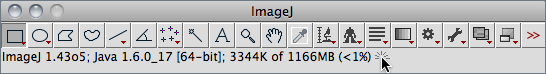
\includegraphics[scale=0.55]{images/StatusBar}
\end{figure}



\calso{\noindent \textsf{\userinterface{\textsf{Plugins\lyxarrow{}Utilities\lyxarrow{}\nameref{sub:ImageJ-Properties...}}},
\userinterface{\textsf{Help\lyxarrow{}\nameref{sub:About-ImageJ...}}}}}

\noindent {\small }
\begin{infobox}
\caption{\label{infobox:Toggle-Cal-Units}Toggling Calibrated Units}


\noindent If a spatial scale has been defined in \userinterface{\noindent Image\lyxarrow{}\nameref{sub:Image>Properties...}}
or \userinterface{\noindent Analyze\lyxarrow{}\nameref{sub:Set-Scale...}},
selection properties are displayed in the \nameref{sub:Status-bar}
in calibrated units. Resizing or moving while holding down \mykeystroke{\noindent Alt}
forces this information to be displayed in pixels.
\end{infobox}
{\small \par}


\subsection*{\noindent Progress bar\label{sub:Progress-bar}}

The \index{Progress bar}progress bar, located to the right of the
status bar, shows the progress of time-consuming operations. It will
not appear if the operation requires less then approximately one second.

%% Momentarily, do not show page numbers for sections in the TOC
\addtocontents{toc}{\protect\cftpagenumbersoff{section}}


\section{Tools\label{sec:IJ-Tools}}

%% Restore defaults
\addtocontents{toc}{\protect\cftpagenumberson{section}}

%% Adjust the lyxlist environment to accomodate the modifier key lists. We'll revert after this section
\renewenvironment{lyxlist}[1]{%
  \begin{list}{}{%
    \settowidth{\labelwidth}{#1}
    \addtolength{\labelwidth}{3.5ex}
    \addtolength{\topsep}{-1.2ex}
    \setlength{\leftmargin}{\labelwidth}
    \addtolength{\leftmargin}{\labelsep}
    \renewcommand{\makelabel}[1]{\qquad{}##1\hfil}
  }%
}{\end{list}}



\subsection{Area Selection Tools\label{sec:Area-selection-tools}}

These tools share the first four toolbar slots. As described in \nameref{sub:Toolbar},
use the right click drop-down menu to switch a different tool. Selection
Color can be changed by double clicking on the \nameref{sec:Point-Tool}/\nameref{sec:Multi-point-Tool}.


\subsubsection[Rectangular Selection Tool]{\noindent \textsf{\protect
\includegraphics[bb=0bp 5bp 20bp 20bp,scale=0.6]{images/tools/Rectangle}}~Rectangular
Selection Tool\label{sub:Rectangular-Selection-Tool}\index{Tools!Area Selection!Rectangle}\index{Rectangular selection}}

\noindent Location, width, height, and aspect ratio are displayed
in the status bar during drawing (\emph{see} \ref{infobox:Toggle-Cal-Units}
\nameref{infobox:Toggle-Cal-Units}).

Modifier keys:
\begin{lyxlist}{00.00.0000}
\item [{\mykeystroke{Shift}}] \noindent Selection is constrained to a
square
\item [{\mykeystroke{Alt}}] \noindent Current \index{Aspect ratio}aspect
ratio is maintained while resizing\\
With arrow keys, width and height are changed one pixel at a time
\item [{\mykeystroke{Ctrl}}] \noindent Selection is resized around the
center
\end{lyxlist}

\calso{\nameref{sub:Round-Rectangular-Selection}, \textsf{\nameref{sub:Specify...}},
\ref{infobox:Color} \nameref{infobox:Color}, \nameref{sub:Tools-shortcuts}}


\subsubsection[Rounded Rectangular Selection Tool]{\noindent \textsf{\protect
\includegraphics[bb=0bp 5bp 20bp 20bp,scale=0.6]{images/tools/RoundRect}}~Rounded
Rectangular Selection Tool\label{sub:Round-Rectangular-Selection}\index{Tools!Area Selection!Rounded Rectangle}\index{Rounded rectangle}\improvement{}}

\noindent %
\begin{minipage}[c][1\totalheight][t]{0.41\columnwidth}%
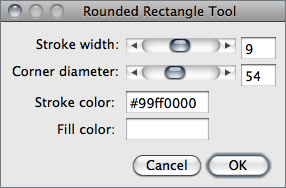
\includegraphics[scale=0.55]{images/RoundRectangle}%
\end{minipage}%
\begin{minipage}[c][1\totalheight][t]{0.59\columnwidth}%
This tool creates rectangular shapes with rounded corners. It shares
the same toolbar slot and the same modifier keys with the \nameref{sub:Rectangular-Selection-Tool}.
Double clicking on its icon opens the depicted dialog in which is
possible to specify:
\begin{description}
\item [{\emph{Stroke\ width}}] The width of the contour.
\item [{\emph{Corner\ diameter}}] The arc size at the vertices.\end{description}
%
\end{minipage}
\begin{description}
\item [{\emph{Stroke/Fill\ Color}}] The contour (stroke) color or the
filling color of the rounded rectangle. As explained in \userinterface{Edit\lyxarrow{}Selection\lyxarrow{}\nameref{sub:Properties...}},
selections can be either filled or contoured, but not both. The nine
default selection colors (\emph{black}, \emph{blue}, \emph{cyan},
\emph{green}, \emph{magenta}, \emph{orange}, \emph{red}, \emph{white},
\emph{yellow}) can be typed as text. Any other color must be typed
in hex notation (\emph{see} \ref{infobox:HEX} \nameref{infobox:HEX}). 
\end{description}

\calso{\nameref{sub:Rectangular-Selection-Tool}, \ref{infobox:Color} \nameref{infobox:Color},
\nameref{sub:Tools-shortcuts}}


\subsubsection[Oval Selection Tool]{\noindent \textsf{\protect
\includegraphics[bb=0bp 5bp 20bp 20bp,scale=0.6]{images/tools/Oval}}~Oval
Selection Tool\label{sub:Oval-Selection-Tool}\index{Tools!Area Selection!Oval}\index{Oval selection}}

\noindent Location, width, height, and aspect ratio are displayed
in the status bar during drawing (\emph{see} \ref{infobox:Toggle-Cal-Units}
\nameref{infobox:Toggle-Cal-Units}).

Modifier keys:
\begin{lyxlist}{00.00.0000}
\item [{\mykeystroke{Shift}}] Selection becomes circular
\item [{\mykeystroke{Alt}}] \noindent Current \index{Aspect ratio}aspect
ratio is maintained while resizing\\
With arrow keys, width and height are changed one pixel at a time
\item [{\mykeystroke{Ctrl}}] Selection is resized around the center
\end{lyxlist}

\calso{\nameref{sub:Elliptical-Selection-Tool}, \textsf{\nameref{sub:Specify...}},
\ref{infobox:Toggle-Cal-Units} \nameref{infobox:Toggle-Cal-Units},
\ref{infobox:Color} \nameref{infobox:Color}, \nameref{sub:Tools-shortcuts}}


\subsubsection[Elliptical Selection Tool]{\noindent \textsf{\protect
\includegraphics[bb=0bp 5bp 20bp 20bp,scale=0.6]{images/tools/Ellipse}}~Elliptical
Selection Tool\label{sub:Elliptical-Selection-Tool}\index{Tools!Area Selection!Ellipse}\index{Elliptical selection}\improvement{}}

Ellipse properties are adjusted by dragging the four handlers on its
antipodal points \cite{C-EllipseTool}. To rotate or resize, drag
the handlers on its major axis (transverse diameter). To adjust eccentricity,
drag the handlers on its minor axis (conjugate diameter). 


\calso{\nameref{sub:Oval-Selection-Tool}, \ref{infobox:Color} \nameref{infobox:Color},
\nameref{sub:Tools-shortcuts}}


\subsubsection[Brush Selection Tool]{\noindent \textsf{\protect
\includegraphics[bb=0bp 5bp 20bp 20bp,scale=0.6]{images/tools/Brush}}~Brush
Selection Tool\label{sub:Brush-Selection-Tool}\index{Tools!Area Selection!Brush}\index{Brush selection tool}\index{Selection!Refine}\improvement{}}

\noindent Adjusts (refines) the shape of area selections using a circular
`brush' \cite{C-ROIbrush}. ImageJ will treat the adjusted ROIs
will become Clicking inside the area selection and dragging along
its boundary will expand the boundary outwards. Clicking outside the
area selection and dragging along its boundary will shrink the boundary
inwards. Once the tool has been applied, ImageJ will treat the adjusted
ROIs as \nameref{sub:Composite-selections}. The brush diameter can
be adjusted by double clicking on the tool icon.

\noindent Modifier keys:
\begin{lyxlist}{00.00.0000}
\item [{\mykeystroke{Shift}}] \noindent Holding Shift forces the Brush
Selection Tool to add pixels to the selection
\item [{\mykeystroke{Alt}}] \noindent Holding Alt forces the Brush Selection
Tool to subtract pixels from the selection
\end{lyxlist}

\calso{\ref{infobox:Composites} \nameref{infobox:Composites}, \nameref{sub:Tools-shortcuts}}


\subsubsection[Polygon Selection Too\textsf{l}]{\noindent \textsf{\protect
\includegraphics[bb=0bp 5bp 20bp 20bp,scale=0.6]{images/tools/Polygon}}~Polygon
Selection Tool\textsf{\label{sub:Polygon-Selection-Tool}}\index{Tools!Area Selection!Polygon}\index{Polygon selection}}

Creates irregularly shaped selections defined by a series of line
segments. Segment length and angle are displayed in the status bar
during drawing (\emph{see} \ref{infobox:Toggle-Cal-Units} \nameref{infobox:Toggle-Cal-Units}).
To create a polygon selection, click repeatedly with the mouse to
create line segments. When finished, click in the small box at the
starting point (or double click), and ImageJ will automatically draw
the last segment. The vertex points that define a polygon selection
can be moved and modifier keys can be used to delete or add new vertexes
to the polygon. 

Modifier keys:
\begin{lyxlist}{00.00.0000}
\item [{\mykeystroke{Shift}}] \noindent Shift-clicking on an existing
vertex of the polygon adds a new corner point, smoothing the polygon
edge
\item [{\mykeystroke{Alt}}] \noindent Alt-clicking on an existing vertex
of the polygon removes it
\end{lyxlist}

\calso{\nameref{sub:Segmented-Line-Selection}, \userinterface{\textsf{\nameref{sub:Enlarge...}}},
\ref{infobox:Toggle-Cal-Units} \nameref{infobox:Toggle-Cal-Units},
\ref{infobox:Color} \nameref{infobox:Color}, \nameref{sub:Tools-shortcuts}}


\subsubsection[Freehand Selection Tool]{\noindent \textsf{\protect
\includegraphics[bb=0bp 5bp 20bp 20bp,scale=0.6]{images/tools/Freehand}}~Freehand
Selection Tool\label{sub:Freehand-Selection-Tool}\index{Tools!Area Selection!Freehand}\index{Freehand area selection}}

As with the polygon selection tool, ImageJ automatically draws the
last segment. Location and intensity of starting pixel are displayed
in the status bar during drawing.


\calso{\nameref{sub:Freehand-Line-Selection}, \nameref{sub:Polygon-Selection-Tool},
\textsf{\userinterface{\textsf{\nameref{sub:Enlarge...}}}}, \ref{infobox:Toggle-Cal-Units}
\nameref{infobox:Toggle-Cal-Units}, \ref{infobox:Color} \nameref{infobox:Color},
\nameref{sub:Tools-shortcuts}}


\subsection{Line Selection Tools\label{sec:Line-Selection-Tools}}

Use these tools to create line selections. The three line selection
tools share the same toolbar slot. As described in \nameref{sub:Toolbar},
use the right click drop-down menu to switch between line tools. 

Double click on any line tool to specify the line width by opening
the \textsf{\userinterface{\textsf{Image\lyxarrow{}Adjust\lyxarrow{}\nameref{sub:Line-WidthSlider}}}}
widget, on which is also possible to apply a cubic spline fit to a
polyline selection. Check the \emph{Sub-pixel resolution} checkbox
in \userinterface{Edit\lyxarrow{}Options\lyxarrow{}\nameref{sub:Profile-Plot-Options...}}
to create line selections with floating-point coordinates (\emph{see}
\nameref{sub:Sub-pixel-Selections}).


\subsubsection[Straight Line Selection Tool]{\protect
\includegraphics[bb=0bp 5bp 20bp 20bp,scale=0.6]{images/tools/StraightLine}~Straight
Line Selection Tool\label{sub:Straight-Line-Selection}}

\index{Tools!Line Selection!Straight Line}\index{Straight line selection}Length
and line angle are displayed in the status bar during drawing (\emph{see}
\ref{infobox:Toggle-Cal-Units} \nameref{infobox:Toggle-Cal-Units}). 

\noindent Modifier keys:
\begin{lyxlist}{00.00.0000}
\item [{\mykeystroke{Shift}}] \noindent Forces the line to be either horizontal
or vertical
\item [{\mykeystroke{Alt}}] \noindent Keeps the line length fixed while
moving either end of the line\\
Forces the two points that define the line to have integer coordinates
when creating a line on a zoomed image
\item [{\mykeystroke{Ctrl}}] \noindent While moving either end of the
line, the line is rotated/resized about its center
\end{lyxlist}

\calso{\textsf{\userinterface{\textsf{\nameref{sub:Calibration-Bar...}}}},
\textsf{\userinterface{\textsf{i\nameref{sub:Set-Scale...}}}}, \ref{infobox:Toggle-Cal-Units}
\nameref{infobox:Toggle-Cal-Units}, \ref{infobox:Color} \nameref{infobox:Color},
\nameref{sub:Tools-shortcuts}}


\subsubsection[Segmented Line Selection Tool]{\protect
\includegraphics[bb=0bp 5bp 20bp 20bp,scale=0.6]{images/tools/SegLine}~Segmented
Line Selection Tool\label{sub:Segmented-Line-Selection}\index{Tools!Line Selection!Segmented Line}\index{Segmented Line selection}\improvement{}}

Works exactly as described for the \nameref{sub:Polygon-Selection-Tool}:
Create a segmented line selection by repeatedly clicking with the
mouse. Each click will define a new line segment. Double click when
finished, or click in the small box at the starting point. The points
that define a segmented line selection can be moved or deleted, and
new points can be added. Length and line angle are displayed in the
status bar during drawing (\emph{see} \nameref{infobox:Toggle-Cal-Units}). 

Modifier keys:
\begin{lyxlist}{00.00.0000}
\item [{\mykeystroke{Shift}}] \noindent Shift-clicking on an existing
vertex adds a new one, adding a new segment to the segmented line
\item [{\mykeystroke{Alt}}] \noindent Alt-clicking on an existing vertex
of the segmented line removes it
\end{lyxlist}

\calso{\nameref{sub:Polygon-Selection-Tool}, \nameref{sub:Freehand-Selection-Tool},
\ref{infobox:Toggle-Cal-Units} \nameref{infobox:Toggle-Cal-Units},
\ref{infobox:Color} \nameref{infobox:Color}, \nameref{sub:Tools-shortcuts}}


\subsubsection[Freehand Line Selection Tool]{\protect
\includegraphics[bb=0bp 5bp 20bp 20bp,scale=0.6]{images/tools/FreehandLine}~Freehand
Line Selection Tool\label{sub:Freehand-Line-Selection}\index{Tools!Line Selection!Freehand Line}\index{Freehand line selection}\improvement{}}

Select this tool and drag with the mouse to create a freehand line
selection.


\calso{\nameref{sub:Freehand-Selection-Tool}, \nameref{sub:OverlayBrush},
\ref{infobox:Toggle-Cal-Units} \nameref{infobox:Toggle-Cal-Units},
\ref{infobox:Color} \nameref{infobox:Color}, \nameref{sub:Tools-shortcuts}}


\subsection[Arrow Tool]{\noindent \protect
\includegraphics[bb=0bp 5bp 20bp 20bp,scale=0.6]{images/tools/Arrow}~Arrow
Tool\label{sec:Arrow-Tool}\textmd{\index{Tools!Line Selection!Arrow}\index{Arrows}\index{Tools!Arrow}}}

\noindent This tool shares the same toolbar slot with the \nameref{sec:Line-Selection-Tools}
and can also be installed on a dedicated toolbar slot using the \nameref{sec:ToolSwitcher}
menu (\emph{see} \nameref{sub:ArrowTool2}). Double clicking on the
tool icon opens its \emph{Options} prompt \cite{C-ArrowTool}. 

\begin{minipage}[c][1\totalheight][t]{0.348\columnwidth}%
\vspace*{15pt}
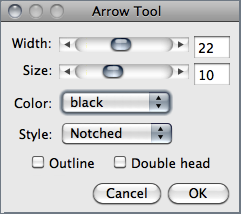
\includegraphics[scale=0.55]{images/ArrowTool}\vspace*{12pt}


\begin{spacing}{0.80000000000000004}
\noindent {\footnotesize }%
\begin{tabular}{>{\raggedright}b{7.8mm}c}
 & {\footnotesize Filled\,\,\ Notched\ \ \,Open}\tabularnewline
{\footnotesize Single head} & {\footnotesize 
\includegraphics[scale=0.65]{images/ArrowTypesS}}\tabularnewline
{\footnotesize Double head} & {\footnotesize 
\includegraphics[scale=0.65]{images/ArrowTypesD}}\tabularnewline
{\footnotesize Outline ~~~} & {\footnotesize 
\includegraphics[scale=0.65]{images/ArrowTypesO}}\tabularnewline
\end{tabular}\end{spacing}
%
\end{minipage}%
\begin{minipage}[c][1\totalheight][t]{0.652\columnwidth}%
Being an \index{Annotations}annotation tool, arrows are created using
foreground color (\emph{see} \textsf{\userinterface{\textsf{\nameref{sub:Color-Picker...[K]}}}})
and not selection color (\emph{see} \nameref{sec:Point-Tool}).

\medskip{}


\emph{Width} and \emph{Size} (in pixels) can be adjusted by dragging
the respective sliders or by direct input. Apart from the arrow styles
listed here, a \emph{Headless} option is also available. As for painting
tools (\nameref{sub:Brush}, \nameref{sub:FloodFiller} and \nameref{sub:Pencil}),
the \emph{Color} dropdown menu provides a convenient way to reset
the foreground color to one of the default options.\medskip{}


\noindent As with any other selection, add arrows to the non-destructive
overlay by pressing \mykeystroke{\noindent B} (\textsf{\userinterface{\noindent \textsf{Image\lyxarrow{}Overlay\lyxarrow{}\nameref{sub:Add-Selection...[b]}}}})
or \mykeystroke{\noindent D} (\textsf{\userinterface{\noindent \textsf{Edit\lyxarrow{}\nameref{sub:Draw-[d]}}}})
to permanently draw the arrow on the image (\emph{see} \ref{infobox:Color}
\nameref{infobox:Color} when working with non-RGB images).\medskip{}


\noindent The same modifier keys described to the \nameref{sub:Straight-Line-Selection}
apply to the arrow tool:%
\end{minipage}.
\begin{lyxlist}{00.00.0000}
\item [{\mykeystroke{Shift}}] \noindent Forces the line to be either horizontal
or vertical
\item [{\mykeystroke{Alt}}] \noindent Keeps the line length fixed while
moving either end of the line\\
Forces the two points that define the line to have integer coordinates
when creating a line on a zoomed image
\item [{\mykeystroke{Ctrl}}] \noindent While moving either end of the
line, the line is rotated/resized about its center
\end{lyxlist}

\calso{\nameref{fig:CPtool}, \ref{infobox:Color} \nameref{infobox:Color},
\nameref{sub:Brush}, \nameref{sub:OverlayBrush}, \nameref{sub:Pencil},
\nameref{sec:Text-Tool}, \nameref{sub:Tools-shortcuts}}


\subsection[Angle Tool]{\noindent \textsf{\protect
\includegraphics[bb=0bp 5bp 20bp 20bp,scale=0.6]{images/tools/Angle}}~Angle
Tool\label{sec:Angle-Tool}\index{Tools!Angle}\index{Angle tool}\index{Reflex angles}}

\sectionmark{Tools}

This tool allows you to measure an angle defined by three points.
Double click on the angle tool icon to enable the measurement of reflex
angles. The angle is displayed in the status bar while the selection
is being created or adjusted. Press \mykeystroke{M} (\textsf{\userinterface{\textsf{Analyze\lyxarrow{}\nameref{sub:Measure...[m]}}}})
to record the angle in the  \nameref{sec:Results-Table}.


\calso{\nameref{sub:Tools-shortcuts}}


\subsection[Point Tool]{\noindent \textsf{\protect
\includegraphics[bb=0bp 5bp 20bp 20bp,scale=0.6]{images/tools/Point}}~Point
Tool\label{sec:Point-Tool}\index{Tools!Point}\index{Point tool}\index{Counting objects}\improvement{}}

Use this tool to create a point selection, to count objects or to
record pixel \index{Coordinates}coordinates.

Modifier keys:
\begin{lyxlist}{00.00.0000}
\item [{\mykeystroke{Shift}}] \noindent Shift-clicking adds more points,
creating a multi-point selection (\emph{see} \nameref{sec:Multi-point-Tool}).
Point count is displayed on the \nameref{sub:Status-bar}
\item [{\mykeystroke{Alt}}] \noindent Alt-clicking on a point deletes
it. Alt-clicking and dragging with the \nameref{sub:Rectangular-Selection-Tool}
or \nameref{sub:Oval-Selection-Tool} deletes multiple points
\end{lyxlist}
\begin{minipage}[c][1\totalheight][t]{0.35\columnwidth}%
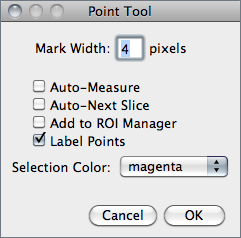
\includegraphics[scale=0.55]{images/PointOptions}%
\end{minipage}%
\begin{minipage}[c][1\totalheight][t]{0.65\columnwidth}%
Double clicking on the point tool icon (or running \textsf{\userinterface{\textsf{Edit\lyxarrow{}Options\lyxarrow{}\nameref{sub:Point-Tool...}}}})
displays its configuration dialog box.
\begin{description}
\item [{\emph{Mark\ Width}}] If greater than zero, a mark of the specified
diameter will be permanently drawn in the current foreground color
(cf.\ \textsf{\userinterface{\textsf{\nameref{sub:Color-Picker...[K]}}}}).
Note that marks modify the image (it may be wise to work with a copy)
and color marks are only available with RGB images (\emph{see} \ref{infobox:Color}
\nameref{infobox:Color}).\end{description}
%
\end{minipage}
\begin{description}
\item [{\emph{Auto-Measure}}] If checked, clicking on the image records
the pixel location and intensity. Note that if \emph{Mark Width} is
not zero, every time a point selection is measured a mark will be
painted (cf.\ \nameref{sub:Measure...[m]}). If unchecked, \userinterface{Edit\lyxarrow{}\nameref{sub:Draw-[d]}}
can be used to paint the mark (\emph{Mark Width }diameter) at the
location of each point.
\item [{\emph{Auto-Next\ Slice}}] If checked, ImageJ will automatically
advance to the next stack slice. Note that this feature will only
allow one point per slice. 
\item [{\emph{Add\ to\ ROI\ Manager}}] If checked, points will be automatically
added to the \nameref{sub:ROI-Manager...}
\item [{\emph{Label\ Points}}] \improvement{}If checked, each point selection
will be displayed with an accompanying numeric label.
\item [{\emph{Selection\ Color}}] Specifies \nameref{sec:Selections-Intro}
color, chosen from one of the nine default colors\emph{: red}, \emph{green},
\emph{blue}, \emph{magenta}, \emph{cyan}, \emph{yellow}, \emph{orange},
\emph{black} and \emph{white}. The chosen color is highlighted in
the center of the Point/MultiPoint Tool. It can also be specified
using \userinterface{Edit\lyxarrow{}Options\lyxarrow{}\nameref{sub:Colors...}}
\end{description}

\calso{\nameref{sec:Multi-point-Tool}, \nameref{lis:ChangeSelectionColor},
\index{Cell Counter plugin}\href{http://imagej.nih.gov/ij/plugins/cell-counter.html}{Cell Counter plugin},
\nameref{sub:Tools-shortcuts}}


\subsection[Multi-point Tool]{\noindent \textsf{\protect
\includegraphics[bb=0bp 5bp 20bp 20bp,scale=0.6]{images/tools/MultiPoint}}~Multi-point
Tool\label{sec:Multi-point-Tool}\index{Tools!Multi-point}\index{Multi-point tool}\index{Counting objects}\improvement{}}

The Multi-point Tool selects multiple points behaving as the \nameref{sec:Point-Tool}
when \mykeystroke{Shift} is pressed,\emph{ Label\ Points} is checked
and \emph{Auto-Measure} and \emph{Auto-Next\ Slice} are deselected.
As described for the \nameref{sec:Point-Tool}, \mykeystroke{Alt}
can also be used to remove points. Similarly, when using \textsf{\userinterface{\textsf{Edit\lyxarrow{}\nameref{sub:Draw-[d]}}}}
marks are painted with the diameter of \emph{Mark Width}. 


\calso{\nameref{sec:Point-Tool}, \index{Cell Counter plugin}\href{http://imagej.nih.gov/ij/plugins/cell-counter.html}{Cell Counter plugin},
\nameref{sub:Tools-shortcuts}}


\subsection[Wand Tool]{\noindent \textsf{\protect
\includegraphics[bb=0bp 5bp 20bp 20bp,scale=0.6]{images/tools/Wand}}~Wand
Tool\label{sub:Wand-Tool}\index{Tools!Area Selection!Wand}\index{Wand tool}\index{Tolerance (Wand Tool)}}

Creates a selection by \index{Tracing@Tracing \see{Wand tool,}}tracing
objects of uniform color or thresholded objects. To trace an object,
either click inside near the right edge, or outside to the left of
the object. To automatically outline and measure objects have a look,
e.g., at the \href{http://imagej.nih.gov/ij/macros/tools/WandAutoMeasureTool.txt}{WandAutoMeasureTool}
macro.

To visualize what happens, imagine a turtle that starts moving to
the right from where you click looking for an edge. Once it finds
the edge, it follows it until it returns to the starting point. Note
that the wand tool may not reliably trace some objects, especially
one pixel wide lines, unless they are thresholded (highlighted in
red) using \textsf{\userinterface{\textsf{Image\lyxarrow{}Adjust\lyxarrow{}\nameref{sub:Threshold...[T]}}}.}

Double clicking on the wand tool icon (or running \textsf{\userinterface{\textsf{Edit\lyxarrow{}Options\lyxarrow{}\nameref{sub:Wand-Tool...}}}})
opens the configuration dialog box in which three modes (4--connected,
8--connected or `Legacy') plus a tolerance value can be set \cite{C-WandTool}.
\begin{figure}[h]
\noindent 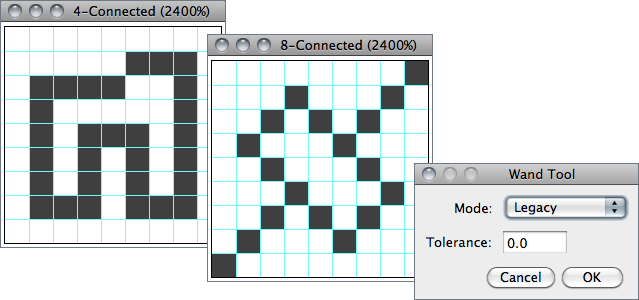
\includegraphics[scale=0.55]{images/WandTool}\caption{\textbf{The \nameref{sub:Wand-Tool}. }4/8--connected particles can
be traced within an intensity range.}
\end{figure}
\textbf{\emph{ }}\phantomsection{}
\begin{description}
\item [{\emph{\label{misc:WandTolerance}Tolerance}}] The wand takes the
pixel value where you click as an initial value. It then selects a
contiguous area under the condition that all pixel values in that
area must be in the range $initial\, value-tolerance$ to $initial\, value+tolerance$.\phantomsection{}
\item [{\emph{\label{misc:Wand4Connected}4--connected}}] Only the four
neighbors of a pixel are considered neighbors. E.g., the wand does
not follow a one-pixel wide diagonal line because the pixels of that
line are not four-connected.\phantomsection{}
\item [{\emph{\label{misc:Wand8Connected}8--connected}}] Each pixel is
considered to have eight neighbors. So the wand follows a diagonal
line if you click onto it. On the other hand, if you have an area
of constant value dissected by a one-pixel wide diagonal line, the
8--connected wand will `jump over the line' and include the other
part of that area.
\item [{\emph{Legacy}}] In this mode no neighbor is checked and no tolerance
is used. This is the default mode of the Wand Tool in ImageJ\,1.42
and earlier.
\end{description}
Modifier keys:
\begin{lyxlist}{00.00.0000}
\item [{\mykeystroke{Shift}}] \noindent Shift-clicking appends the traced
area to previously traced selections
\item [{\mykeystroke{Alt}}] \noindent Alt-clicking removes the traced
area from previously traced selections
\end{lyxlist}

\calso{\userinterface{Analyze\lyxarrow{}\nameref{sub:Analyze-Particles...}},
\nameref{sub:FloodFiller}, \nameref{sub:Composite-selections}, \nameref{sub:Tools-shortcuts}}


\subsection[Text Tool]{\noindent \textsf{\protect
\includegraphics[bb=0bp 5bp 20bp 20bp,scale=0.6]{images/tools/Text}}~Text
Tool\label{sec:Text-Tool}\index{Tools!Text}\index{Text}\index{Annotations}}

\begin{minipage}[c][1\totalheight][t]{0.3\columnwidth}%
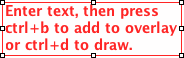
\includegraphics[scale=0.6]{images/TextTool}%
\end{minipage}%
\begin{minipage}[c][1\totalheight][t]{0.7\columnwidth}%
Use this tool to add text to images. It creates text ROIs, rectangular
selections containing one or more lines of text. Note the following
when using the Text Tool: %
\end{minipage}
\begin{itemize}
\item Font style and text alignment is specified in the \emph{Fonts} widget,
activated by double clicking on 
\includegraphics[bb=0bp 5bp 20bp 20bp,scale=0.6]{images/tools/Text}
or by running \userinterface{Edit\lyxarrow{}Options\lyxarrow{}\nameref{sub:Fonts...}}
Text is drawn in foreground color (\emph{see} \nameref{sub:Color-Picker...[K]})
\item Use the keyboard to add characters to the text and the backspace key
to delete characters. Use \mykeystroke{Alt} to type special unit
symbols such as $\micro$ (\mykeystroke{Alt}\mykeystroke{M}) or
$\angstrom$ (\mykeystroke{Alt}\mykeystroke{Shift}\mykeystroke{A}).
Note that menu shortcuts require holding down \mykeystroke{Ctrl}
while using the Text Tool (\emph{see} \nameref{sub:Using-Shortcuts})
\item Use \mykeystroke{Ctrl}\mykeystroke{Y} (\userinterface{Edit\lyxarrow{}Selection\lyxarrow{}\nameref{sub:Properties...}})
to re-adjust font color and size, text justification and to specify
a background color for the text selection. \ref{infobox:HEX} \nameref{infobox:HEX}
provides instructions on how to define semi-transparent colored backgrounds
(\emph{see also} \filenameref{\href{http://imagej.nih.gov/ij/macros/examples/DrawTextWithBackground.txt}{DrawTextWithBackground}}
macro)
\item Use \mykeystroke{Ctrl}\mykeystroke{B} (\userinterface{Image\lyxarrow{}Overlay\lyxarrow{}\nameref{sub:Add-Selection...[b]}})
to create non-destructive text annotations (\emph{see} \nameref{sub:Overlay-Intro};
\filenameref{\href{http://imagej.nih.gov/ij/macros/examples/OverlayDrawStringDemo.txt}{OverlayDrawStringDemo}},
\filenameref{\href{http://imagej.nih.gov/ij/macros/examples/TextOverlay.txt}{TextOverlay}}
macros). Alternatively, use \mykeystroke{Ctrl}\mykeystroke{D} (\userinterface{Edit\lyxarrow{}\nameref{sub:Draw-[d]}})
to permanently draw the text on the image. In the latter case, the
background of the text selection is not drawn (\emph{see also} \ref{infobox:Color}
\nameref{infobox:Color})
\end{itemize}

\calso{\nameref{sec:Arrow-Tool}, \nameref{sub:Brush}, \nameref{sub:OverlayBrush},
\nameref{sub:Pencil}, \filenameref{\href{http://imagej.nih.gov/ij/macros/TextDemo.txt}{TextDemo}}
macro, \nameref{sub:Tools-shortcuts} }


\subsection[Magnifying Glass]{\noindent \textsf{\protect
\includegraphics[bb=0bp 5bp 20bp 20bp,scale=0.6]{images/tools/Glass}}~Magnifying
Glass\label{sec:Magnifying-Glass}\index{Tools!Magnifying Glass}\index{Magnifying Glass Tool}}

Magnifies and reduces the view of active image. Activate the tool
and click on the image \index{Zoom}zoom in. Right-click (or Alt-click)
to zoom out. The current magnification is shown in the image's title
bar. Double click on the magnifying glass icon to revert to the image's
original magnification. As explained in \textsf{\userinterface{Image\lyxarrow{}Zoom\lyxarrow{}\nameref{sub:ZoomIn}}},
there are 21 possible magnification levels: 3.1, 4.2, 6.3, 8.3, 12.5,
16.7, 25, 33.3, 50, 75, 100, 150, 200, 300, 400, 600, 800, 1200, 1600,
2400 and 3200\%. 

Modifier keys:
\begin{lyxlist}{00.00.0000}
\item [{\mykeystroke{Shift}}] \noindent Clicking and dragging while holding
down the Shift key runs \textsf{\userinterface{Image\lyxarrow{}Zoom\lyxarrow{}\nameref{sub:ZoomToSelection}}}
\item [{\mykeystroke{Alt}}] \noindent Image zooms out (right-click behavior)
\end{lyxlist}

\calso{\ref{infobox:ZoomedCanvas} \nameref{infobox:ZoomedCanvas}\textsf{,
\userinterface{\textsf{\nameref{sub:Zoom}}}} commands, \nameref{sub:Tools-shortcuts}}


\subsection[Scrolling Tool]{\noindent \textsf{\protect
\includegraphics[bb=0bp 5bp 20bp 20bp,scale=0.6]{images/tools/Hand}}~Scrolling
Tool\label{sec:Scrolling-Tool}\index{Tools!Scrolling}\index{Scrolling}}

Allows you to scroll through an image that is larger than its window.
You can temporarily activate this tool (except when using the \nameref{sec:Text-Tool})
by holding down the space bar.


\calso{\ref{infobox:ZoomedCanvas} \nameref{infobox:ZoomedCanvas}, \nameref{sub:Tools-shortcuts}}


\subsection[Color Picker Tool]{\noindent \textsf{\protect
\includegraphics[bb=0bp 5bp 20bp 20bp,scale=0.6]{images/tools/ColorPicker}}~Color
Picker\label{sec:Color-Picker}\index{Tools!Color Picker}\index{Color Picker}\index{Eye dropper}}

Sets the foreground drawing color by `picking up' colors from any
open image. Colors can also be picked up from the Color Picker (CP\nomenclature{CP}{Color Picker})
window (\textsf{\userinterface{\textsf{Image\lyxarrow{}Colors\lyxarrow{}}\nameref{sub:Color-Picker...[K]}}})
using any tool. In the icon, the `eye dropper' is drawn in the current
\index{Color!Foreground}foreground color while the frame around it
is drawn in the current \index{Color!Background}background color.
\userinterface{\textsf{Edit\lyxarrow{}}\nameref{sub:Draw-[d]}} and
\textsf{\userinterface{\textsf{Edit\lyxarrow{}}\nameref{sub:Fill-[f]}}}
use the foreground color. \textsf{\userinterface{\textsf{Edit\lyxarrow{}}\nameref{sub:Clear}}},
\userinterface{\nameref{sub:Clear-Outside}} and\textsf{ \userinterface{\textsf{\nameref{sub:Cut[x]}}}}
use the background color. Double clicking on the tool icon will display
the Color Picker window. 

Modifier key:
\begin{lyxlist}{00.00.0000}
\item [{\mykeystroke{Alt}}] \noindent Alt-clicking with the Color Picker
Tool on the image canvas `picks-up' background color 
\end{lyxlist}

\calso{\nameref{fig:CPtool}, \ref{infobox:Color} \nameref{infobox:Color},
\nameref{sub:Tools-shortcuts}, \nameref{lis:toolsShrtct3}}


\subsection[\emph{More Tools} Menu]{\noindent \textsf{\protect
\includegraphics[bb=0bp 5bp 20bp 20bp,scale=0.6]{images/tools/Switcher}}~\emph{More
Tools} Menu\label{sec:ToolSwitcher}\improvement{}\change{}}

The eight \nameref{sub:Toolbar} slots between the \nameref{sec:Color-Picker}
and the \emph{More Tools} Menu\index{Tools!More Tools Menu@\emph{More Tools} Menu}\index{More Tools Menu@\emph{More Tools} Menu}\index{Tools!Toolset Switcher@Toolset Switcher \see{\emph{More Tools} Menu,}}
can be customized using this drop-down menu (named \emph{Toolset Switcher}
in previous IJ versions). Tool configurations are stored in the ImageJ
preferences file (\emph{see} \nameref{sec:Settings-and-Preferences})
and retrieved across restarts. 

The \nameref{fig:MoreToolsList} is populated by \filenameref{\noindent StartupMacros.txt}
in \dirnameref{ImageJ/macros/}, \nameref{misc:Toolsets} installed
in \dirnameref{ImageJ/macros/toolsets/}, built-in tools loaded from
\filenameref{ij.jar} (\nameref{sub:ArrowTool2}, \nameref{sub:Brush},
\nameref{sub:DevMenu}, \nameref{sub:FloodFiller}, \nameref{sub:LUTMenu},
\nameref{sub:OverlayBrush}, \nameref{sub:Pencil}, \nameref{sub:SprayCan}
and \nameref{sub:StacksMenu}) and \nameref{misc:CustomSingleTools}
installed in \dirnameref{ImageJ/plugins/Tools/}.

At startup, the default set of tools is typically loaded from \index{StartupMacros}\filenameref{StartupMacros.txt}.
Later on, tools can be appended or replaced. \nameref{misc:CustomSingleTools}
are installed in the first available slot, or in the last slot if
no free slots are available\index{Toolsets}. \nameref{misc:Toolsets}
replace all the eight slots in the toolbar. Choose \emph{Remove Tool}s
to reset the toolbar. 

The icons for drawing tools installed from this menu reflect the foreground
color (\emph{see} \nameref{sub:Color-Picker...[K]}) and are updated
when the foreground color changes. 

Modifier key:
\begin{lyxlist}{00.00.0000}
\item [{\mykeystroke{Shift}}] \noindent Shift-clicking on the menu icon
will open the selected macro (\filenameref{.txt} and \filenameref{.ijm}
files)
\end{lyxlist}

\calso{\nameref{sec:CustomToolsAndToolsets}, \nameref{sub:Tools-shortcuts}}

\begin{figure}
\noindent {\small 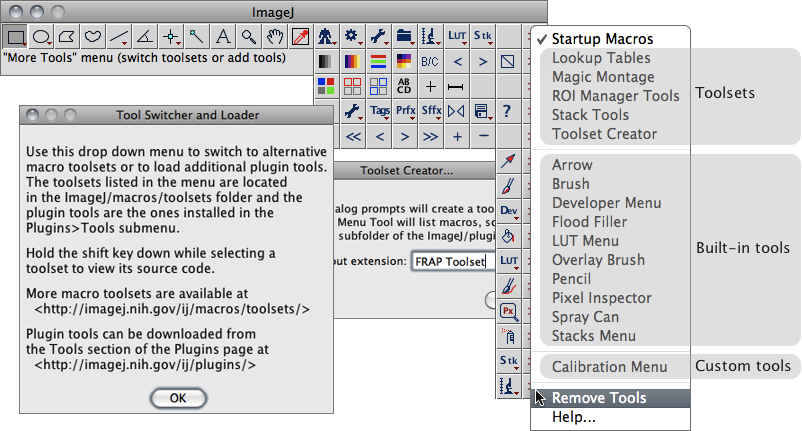
\includegraphics[scale=0.55]{images/MoreToolsMenu}}\caption[\emph{More Tools} list]{\label{fig:MoreToolsList}\textbf{\nameref{sec:ToolSwitcher} (IJ\,1.46n).}
The menu lists tools from \protect\filenameref{\noindent StartupMacros.txt}
in \protect\dirnameref{ImageJ/macros/}, \nameref{misc:Toolsets}
installed in \protect\dirnameref{ImageJ/macros/toolsets/}, built-in
tools loaded from \protect\filenameref{ij.jar} (\nameref{sub:ArrowTool2},
\nameref{sub:Brush}, \nameref{sub:DevMenu}, \nameref{sub:FloodFiller},
\nameref{sub:LUTMenu}, \nameref{sub:OverlayBrush}, \nameref{sub:Pencil},
\nameref{sub:SprayCan} and \nameref{sub:StacksMenu}) and \nameref{misc:CustomSingleTools}
installed in \protect\dirnameref{ImageJ/plugins/Tools/}. While toolsets
replace all the eight slots in the toolbar, single tools are installed
in the first available slot, or in the last slot if no free slots
are available.}
\end{figure}



\subsection[Arrow]{\noindent \textsf{\protect
\includegraphics[bb=0bp 5bp 20bp 20bp,scale=0.6]{images/tools/Switcher}}~\textsf{\protect
\includegraphics[bb=0bp 5bp 20bp 20bp,scale=0.6]{images/tools/Arrow2}}~Arrow\textmd{\index{Tools!Arrow}\index{Arrows}}\label{sub:ArrowTool2}\textmd{\index{Tools!Line Selection!Arrow}\index{Arrows}\index{Tools!Arrow}}\feature{}}

Installs a copy of the \nameref{sec:Arrow-Tool} on the first available
toolbar slot (or the last if no free slots are available), so that
it can be accessed without the need of selecting it on the \nameref{sec:Line-Selection-Tools}
dropdown menu. Refer to the original \nameref{sec:Arrow-Tool} for
details and modifier keys.


\calso{\nameref{fig:CPtool}, \ref{infobox:Color} \nameref{infobox:Color},
\nameref{sub:Brush}, \nameref{sub:OverlayBrush}, \nameref{sub:Pencil},
\nameref{sec:Text-Tool}, \nameref{sub:Tools-shortcuts}}


\subsection[Brush]{\noindent \textsf{\protect
\includegraphics[bb=0bp 5bp 20bp 20bp,scale=0.6]{images/tools/Switcher}}~\textsf{\protect
\includegraphics[bb=0bp 5bp 20bp 20bp,scale=0.6]{images/tools/Brush1}}~Brush\label{sub:Brush}\feature{New tools: Arrow, Brush, Developer Menu, Flood Filler, LUT Menu, Overlay Brush, Pencil, Pixel Inspector, Spray Can and Stacks Menu}}

\begin{minipage}[c][1\totalheight][t]{0.667\columnwidth}%
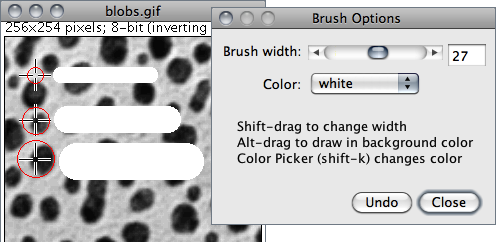
\includegraphics[scale=0.55]{images/Brush}%
\end{minipage}%
\begin{minipage}[c][1\totalheight][t]{0.333\columnwidth}%
A freehand \index{Brush}\index{Tools!Brush}\index{Paintbrush@Paintbrush \see{Brush and Overlay Brush,}}paintbrush
tool that draws invasively (as opposed to the \nameref{sub:OverlayBrush}
that draws on a non-destructive image overlay (\emph{see} \nameref{sub:Overlay-Intro}
and \userinterface{Image\lyxarrow{}\nameref{sub:Overlay}} commands).\medskip{}


Double clicking on the tool icon opens its \emph{Options} dialog box
in which is possible to specify the \emph{Brush width} (in pixels)
and \emph{Color}.%
\end{minipage}

Being an \index{Annotations}annotation tool, the paintbrush paints
in foreground color as reflected its icon (\emph{see} \ref{infobox:Color}
\nameref{infobox:Color} when working with non-RGB images). The \emph{Color}
dropdown menu provides a convenient way to reset the foreground color
to one of the default options, bypassing the need of opening the \nameref{fig:CPtool},
evoked using \mykeystroke{Ctrl} \mykeystroke{K}.\emph{ }As previously
described (\emph{see} \nameref{sec:Undo-and-Redo}), undo is restricted
to last drawing step. The Brush and \nameref{sub:Pencil} tools are
in all similar, differing only on brush (stroke) size.

Modifier keys:
\begin{lyxlist}{00.00.0000}
\item [{\mykeystroke{Shift}}] \noindent Shift-dragging on the canvas will
adjust the brush size
\item [{\mykeystroke{Alt}}] \noindent Holding Alt makes the brush paint
in background color 
\end{lyxlist}

\calso{\nameref{sub:OverlayBrush}, \nameref{sub:Pencil}, \nameref{sub:Freehand-Line-Selection},
\nameref{fig:CPtool}, \ref{infobox:Color} \nameref{infobox:Color},
\nameref{sub:Tools-shortcuts}}


\subsection[Developer Menu]{\noindent \textsf{\protect
\includegraphics[bb=0bp 5bp 20bp 20bp,scale=0.6]{images/tools/Switcher}}~\textsf{\protect
\includegraphics[bb=0bp 5bp 20bp 20bp,scale=0.6]{images/tools/DevMenu}}~Developer
Menu\label{sub:DevMenu}\index{Developer Menu}\index{Tools!Developer Menu}\feature{}}

A drop-down menu collecting several online resources and commands
that are useful when writing \nameref{sub:Macros-ExtendingIJ}, \nameref{sub:Plugins}
or troubleshooting ImageJ operations.

\emph{Debug mode} activates ImageJ's debugging mode (\userinterface{Edit\lyxarrow{}Options\lyxarrow{}\nameref{sub:Misc...}}).


\calso{\nameref{sec:Extending-ImageJ}, \nameref{sub:ImageJ-Macro-Editor},
\userinterface{\nameref{sec:Help}}, \userinterface{Plugins\lyxarrow{}\nameref{sub:Macros}}/\userinterface{\nameref{sub:Utilities}}/\userinterface{\nameref{sub:Plugins->New}},
\href{http://rsbweb.nih.gov/ij/plugins/cc-menu/index.html}{Common Commands Menu Tool},
\nameref{sub:StacksMenu}, \nameref{sub:LUTMenu}}


\subsection[Flood Filler]{\noindent \textsf{\protect
\includegraphics[bb=0bp 5bp 20bp 20bp,scale=0.6]{images/tools/Switcher}}~\textsf{\protect
\includegraphics[bb=0bp 5bp 20bp 20bp,scale=0.6]{images/tools/FloodFiller}}~Flood
Filler\label{sub:FloodFiller}\index{Flood Filler}\index{Tools!Flood Filler}\feature{}}

A \index{Paint Bucket Tool@Paint Bucket Tool \see{Flood Filler,}}\emph{paint
bucket }tool that fills with the current foreground color adjacent
pixels that have the same value as the clicked pixel. Double click
on the tool icon to specify the \href{http://en.wikipedia.org/wiki/Flood_fill}{flood type}
in terms of pixel connectivity: \nameref{misc:Wand4Connected} or
\nameref{misc:Wand8Connected}.

To spread the fill to contiguous pixels within an intensity range,
use the \nameref{sub:Wand-Tool} instead: Double click on the Wand
Tool icon to set a \nameref{misc:WandTolerance} value, then press
\mykeystroke{F} (\userinterface{Edit\lyxarrow{}\nameref{sub:Fill-[f]}})
to fill with foreground color (highlighted in the Flood Filler icon)
or \mykeystroke{Backspace}/\mykeystroke{Del} (\userinterface{Edit\lyxarrow{}\nameref{sub:Clear}})
to fill with background color (\emph{see} \userinterface{\nameref{sub:Color-Picker...[K]}}).

Modifier keys:
\begin{lyxlist}{00.00.0000}
\item [{\mykeystroke{Alt}}] \noindent Alt-clicking makes the brush paint
in background color
\end{lyxlist}

\calso{\code{\href{http://imagej.nih.gov/ij/developer/macro/functions.html\#floodFill}{floodFill(x,y)}}
macro function, \nameref{fig:CPtool}, \ref{infobox:Color} \nameref{infobox:Color},
\nameref{sub:Tools-shortcuts}}


\subsection[LUT Menu]{\noindent \textsf{\protect
\includegraphics[bb=0bp 5bp 20bp 20bp,scale=0.6]{images/tools/Switcher}}~\textsf{\protect
\includegraphics[bb=0bp 5bp 20bp 20bp,scale=0.6]{images/tools/LUTMenu}}~LUT
Menu\label{sub:LUTMenu}\index{LUT Menu}\index{Tools!LUT Menu}\feature{}}

A drop-down menu listing all the \userinterface{Image\lyxarrow{}\nameref{sub:Lookup-Tables}}
commands. It is a convenient way to deal with a large collection of
lookup tables that otherwise would only be accessed through the menu
bar. Note that although it is not possible to organize LUTs into subfolders,
it is possible to rename the most frequently used lookup tables with
a numeric prefix (e.g, \filenameref{\href{http://imagej.nih.gov/ij/download/luts/glasbey.lut}{01-glasbey.lut}},
\filenameref{\href{http://imagej.nih.gov/ij/download/luts/thermal.lut}{02-Termal.lut}},
etc.) so that they are listed earlier in the menu.


\calso{\nameref{sub:Pseudocolor-Images}, \filenameref{\href{http://imagej.nih.gov/ij/macros/Show_All_LUTs.txt}{Show\_{}All\_{}LUTs}}
(a macro that creates a \href{http://imagej.nih.gov/ij/download/luts/LUT_Montage.jpg}{graphical palette}
of all the installed lookup tables), \nameref{sub:StacksMenu}, \href{http://rsbweb.nih.gov/ij/plugins/cc-menu/index.html}{Common Commands Menu Tool},
\nameref{sub:DevMenu}}


\subsection[Overlay Brush]{\noindent \textsf{\protect
\includegraphics[bb=0bp 5bp 20bp 20bp,scale=0.6]{images/tools/Switcher}}~\textsf{\protect
\includegraphics[bb=0bp 5bp 20bp 20bp,scale=0.6]{images/tools/Brush2}}~Overlay
Brush\label{sub:OverlayBrush}\index{Overlay Brush}\index{Tools!Overlay Brush}\index{Annotations}\feature{}}

\begin{minipage}[c][1\totalheight][t]{0.645\columnwidth}%
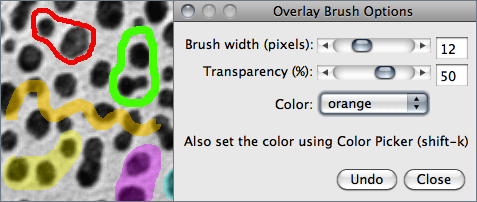
\includegraphics[scale=0.55]{images/OverlayBrush}%
\end{minipage}%
\begin{minipage}[c][1\totalheight][t]{0.355\columnwidth}%
A freehand paintbrush that draws on a non-destructive image overlay
(\emph{see} \nameref{sub:Overlay-Intro}), as opposed to the \nameref{sub:Brush}
tool that draws invasively over the canvas.\medskip{}


Double clicking on the tool icon opens its \emph{Options} dialog box
in which is possible to specify the \emph{Brush width} (in pixels),
\emph{Transparency (\%)} and \emph{Color}.%
\end{minipage}

As previously described (\emph{see} \nameref{sub:Brush} and \nameref{sub:Pencil}
tools), the \emph{Color} dropdown menu changes the foreground color,
bypassing the \nameref{fig:CPtool} (activated by \mykeystroke{Ctrl}
\mykeystroke{K}). Press \emph{Undo} to remove the last painted stroke
from the overlay. Overlay manipulations are described in \userinterface{Image\lyxarrow{}\nameref{sub:Overlay}}.


\calso{\nameref{sub:Freehand-Line-Selection}, \ref{infobox:Color} \nameref{infobox:Color},
\nameref{sub:Tools-shortcuts}}


\subsection[Pencil]{\noindent \textsf{\protect
\includegraphics[bb=0bp 5bp 20bp 20bp,scale=0.6]{images/tools/Switcher}}~\textsf{\protect
\includegraphics[bb=0bp 5bp 20bp 20bp,scale=0.6]{images/tools/Pencil}}~Pencil\label{sub:Pencil}\index{Pencil}\index{Tools!Pencil}\feature{}}

A freehand painting tool that draws invasively in foreground color.
It is in all similar to the \nameref{sub:Brush} tool but it is typically
used with thinner strokes. Double clicking on the tool icon opens
its \emph{Options} dialog box in which is possible to specify the
\emph{Pencil width} (in pixels) and \emph{Color}. Refer to the \nameref{sub:Brush}
tool tools for details.

Modifier keys:
\begin{lyxlist}{00.00.0000}
\item [{\mykeystroke{Shift}}] \noindent Shift-dragging on the canvas will
adjust the brush size
\item [{\mykeystroke{Alt}}] \noindent Holding Alt makes the brush paint
in background color (\emph{see} \userinterface{\nameref{sub:Color-Picker...[K]}})
\end{lyxlist}

\calso{\nameref{sub:Freehand-Line-Selection}, \nameref{sub:OverlayBrush},
\nameref{fig:CPtool}, \ref{infobox:Color} \nameref{infobox:Color},
\nameref{sub:Tools-shortcuts}}


\subsection[Pixel Inspector]{\noindent \textsf{\protect
\includegraphics[bb=0bp 5bp 20bp 20bp,scale=0.6]{images/tools/Switcher}}~\textsf{\protect\includegraphics[bb=0bp 5bp 20bp 20bp,scale=0.6]{images/tools/Inspector}}~Pixel
Inspector\textmd{\index{Tools!Pixel Inspector}\index{Pixel Inspector}}\label{sub:PixelInspector}\feature{}}

\begin{minipage}[c][1\totalheight][t]{0.605\columnwidth}%
\includegraphics[scale=0.55]{images/PixelInspector}%
\end{minipage}%
\begin{minipage}[c][1\totalheight][t]{0.395\columnwidth}%
The Pixel inspector displays the values of a square neighborhood around
the current cursor position as a table \cite{C-PixelInspector}. Values
are updated in real time as the mouse is dragged over the image. It
is useful to examine how a filter changes the pixel data. E.g., load
Pixel Inspector, move the cursor over an image and run \userinterface{Process\lyxarrow{}Filters\lyxarrow{}\nameref{sub:Gaussian-Blur...}}:
When toggling the \emph{Preview} checkbox you will be able to monitor
in real time how different \emph{Sigma} radius change pixel values.%
\end{minipage}

In the \emph{Pixel Values} table, columns and row headers (x \& y
positions) are expressed in pixel coordinates. The y-axis direction
is determined by the \nameref{misc:InvertYcoordinates} value in \userinterface{Analyze\lyxarrow{}\nameref{sub:Set-Measurements...}}
The center position (current cursor) is printed in red (\emph{x},
\emph{y}, \emph{value}). When the table is in the foreground, the
arrow keys can be used to nudge the neighborhood square (outlined
in red) and the table can be copied into the clipboard by pressing
\mykeystroke{C}. For settings, press the \emph{Prefs} button at the
top left of the table:
\begin{description}
\item [{\emph{Radius}}] Specifies the size of the table, $3\times3$ for
$radius=1$;  $5\times5$ for $radius=2$, etc. 
\item [{\emph{Grayscale\ readout}}] The numeric output for 8 and 16--bit
grayscale images. Can be\emph{ Raw} {[}the default{]}, \emph{Calibrated}
{[}\emph{see} \userinterface{Analyze\lyxarrow{}\nameref{sub:Calibrate...}}{]}
or Hexadecimal (\emph{Hex}).
\item [{\emph{RGB\ readout}}] The numeric output for RGB images. Can be
\emph{R,G,B} triplets, \emph{Gray Value} or Hexadecimal (\emph{Hex})
{[}\emph{see} \ref{infobox:HEX} \nameref{infobox:HEX}{]}. The mean
grayscale value is determined by the weighting factors specified in
\userinterface{Edit\lyxarrow{}Options\lyxarrow{}\nameref{sub:Conversions...}}
\item [{\emph{Copy\ to\ clipboard}}] Specifies which data is copied to
the clipboard. Choose \emph{Data only} to copy the table without headers,
\emph{x,y and Data} to copy the current position (x,y) values followed
by remaining data or \emph{Header and Data} to copy the table with
headers. Tables are copied as tab-delimited values.
\end{description}

\calso{\nameref{fig:TextImages}, \userinterface{Image\lyxarrow{}Transform\lyxarrow{}\nameref{sub:ImageToResults}/\nameref{sub:ResultsToImage}},
\userinterface{File\lyxarrow{}Save As\lyxarrow{}\nameref{sub:SaveAs>Text-Image...}},
\userinterface{Import\lyxarrow{}\nameref{sub:Import>Text-Image}},
\nameref{sub:Tools-shortcuts}}


\subsection[Spray Can]{\noindent \textsf{\protect\includegraphics[bb=0bp 5bp 20bp 20bp,scale=0.6]{images/tools/Switcher}}~\textsf{\protect\includegraphics[bb=0bp 5bp 20bp 20bp,scale=0.6]{images/tools/SprayCan}}~Spray
Can\label{sub:SprayCan}\feature{}}

The \index{Tools!Spray Can}\index{Spray Can}\index{Noise}Spray
Can (\emph{Airbrush} tool) draws random pixels in the current foreground
color (\emph{paint}) (\emph{see} \nameref{sub:Color-Picker...[K]}
and \ref{infobox:Color} \nameref{infobox:Color}). It behaves as
a traditional airbrush or spray paint: Holding the main mouse button
(without moving the cursor) will build up \emph{paint}, as if pressing
the nozzle of an aerosol paint can.\emph{ Spray widt}h,\emph{ Dot
size} and \emph{Flow rat}e can be specified by double clicking on
the tool icon.

This tool is useful to generate random spot noise. Use it to, e.g.,
assess the effectiveness of median filtering: Load the Spray Can tool,
apply it over an image and toggle the \emph{Preview} option in the
\userinterface{Process\lyxarrow{}Filters\lyxarrow{}\nameref{sub:Median...}}
prompt. 


\calso{\userinterface{Process\lyxarrow{}Noise\lyxarrow{}\nameref{sub:Add-Noise}},
\userinterface{\nameref{sub:Salt-and-Pepper}}, \nameref{sub:Tools-shortcuts}}


\subsection[Stacks Menu]{\noindent \textsf{\protect\includegraphics[bb=0bp 5bp 20bp 20bp,scale=0.6]{images/tools/Switcher}}~\textsf{\protect\includegraphics[bb=0bp 5bp 20bp 20bp,scale=0.6]{images/tools/StacksMenu}}~Stacks
Menu\label{sub:StacksMenu}\index{Stacks Menu}\index{Tools!Stacks Menu}\feature{}}

A drop-down menu collecting several commands related to \nameref{sub:Stacks-Intro}
and \nameref{sub:Hyperstacks-Intro}, otherwise accessed through the
hierarchy of \userinterface{Image\lyxarrow{}\nameref{sub:Stacks}},
\userinterface{Image\lyxarrow{}\nameref{sub:Hyperstacks}} and \userinterface{File\lyxarrow{}\nameref{sub:OpenSamples}}submenus.
The list makes a particular emphasis on commands that have no keyboard
shortcuts assigned.


\calso{\userinterface{Plugins\lyxarrow{}\nameref{sub:Shortcuts}}, \nameref{sub:LUTMenu},
\nameref{sub:StacksMenu}, \href{http://rsbweb.nih.gov/ij/plugins/cc-menu/index.html}{Common Commands Menu Tool},
\nameref{sub:DevMenu}}

%% Restore the lyxlist environment to its defaults
\renewenvironment{lyxlist}[1]{%
  \begin{list}{}{%
    \settowidth{\labelwidth}{#1}
    \setlength{\leftmargin}{\labelwidth}
    \addtolength{\leftmargin}{\labelsep}
    \renewcommand{\makelabel}[1]{##1\hfil}
  }%
}{\end{list}}



\section{\noindent Custom Tools\index{Tools!Custom tools}\index{Macro tools}\index{Plugin tools}\label{sec:CustomToolsAndToolsets}}

Customized tools are add-ons (macros and plugins) that allow custom
interactions with the ImageJ toolbar and/or the image canvas. They
are installed on the right side of the \nameref{sub:Toolbar} between
the \nameref{sec:Color-Picker} and the \nameref{sec:ToolSwitcher}.
At startup, the default set of tools is loaded from \index{StartupMacros}\filenameref{ImageJ/macros/StartupMacros.txt}.
Later on, tools can be appended or replaced using the \nameref{sec:ToolSwitcher}
menu. As mentioned, custom tool configurations are saved in the preferences
file, and thus remembered across restarts (\emph{see} \nameref{sec:Settings-and-Preferences}).

It is worth it to mention some differences between the installation
of single tools and toolsets:
\begin{description}
\item [{Single\ Tools\label{misc:CustomSingleTools}}] \index{Tools!Plugin Tools}\index{Plugin Tools}
Single tools are appended to the first available toolbar slot or installed
in the last slot if no free slots are available. Tools can be macros
(\filenameref{.txt} and \filenameref{.ijm} files) or \feature{Plugin Tools} \negthinspace{}\negthinspace{}plugins
(\filenameref{.class} and \filenameref{.jar} files) and are listed
on the \nameref{sec:ToolSwitcher} menu if placed in the \dirnameref{ImageJ/plugins/Tools/}
directory. In addition to the macro tools distributed with ImageJ
and saved in \dirnameref{ImageJ/macros/tools/}, a vast repertoire
of \href{http://imagej.nih.gov/ij/plugins/index.html\#tools}{tools}
is available on the ImageJ website.
\item [{Toolsets\label{misc:Toolsets}}] \index{Toolsets}Toolsets are
macro files (\filenameref{.txt} and \filenameref{.ijm} files) containing
up to eight macro tools, along with any number of ordinary macros.
Toolsets are listed on the \nameref{sec:ToolSwitcher} menu if installed
in the \dirnameref{ImageJ/macros/toolsets/} directory. Choosing a
toolset (e.g., \emph{Lookup Tables}) replaces all previously installed
tools. \\
As mentioned, \index{StartupMacros}\filenameref{ImageJ/macros/StartupMacros.txt}
contains the tools loaded at startup. This file can be customized
using \userinterface{Plugins\lyxarrow{}Macros\lyxarrow{}\nameref{sub:Startup-Macros...}}
or by holding \mykeystroke{Shift} when choosing \emph{Startup Macros}
from the \nameref{sec:ToolSwitcher} menu. \\
ImageJ feature several pre-installed toolsets \cite{C-Toolsets} and
many others are available on the \href{http://imagej.nih.gov/ij/plugins/index.html\#toolsets}{ImageJ website}.
Toolsets can also be created by choosing \emph{Toolset Creator}, a
convenient way to create groups of Menu Tools listing \userinterface{\nameref{sec:Plugins}}
commands.
\end{description}

\calso{\nameref{sec:ToolSwitcher}, \href{http://imagej.nih.gov/ij/developer/macro/macros.html\#tools}{Tools documentation},
\userinterface{Plugins\lyxarrow{}New\lyxarrow{}\nameref{sub:NewMacroTool}},
\userinterface{\nameref{sub:NewPluginTool}}}


\section[Contextual Menu]{Contextual Menu\label{sec:ContextualMenu}}

\begin{minipage}[c][1\totalheight][t]{0.413\columnwidth}%
\includegraphics[scale=0.55]{images/PopupMenu}%
\end{minipage}%
\begin{minipage}[c][1\totalheight][t]{0.587\columnwidth}%
As mentioned earlier macros and macro tools in the\texttt{ }\index{StartupMacros}\filenameref{StartupMacros.txt}
are automatically installed in the \textsf{\userinterface{\textsf{Plugins\lyxarrow{}Macros\lyxarrow{}}}
}submenu and in the toolbar when ImageJ starts up. 

\medskip{}
In addition, the \filenameref{StartupMacros.txt} file also installs
the \index{Contextual Menu}contextual (\index{Pop-up menu@Pop-up menu  \see{Contextual menu,}}popup)
menu displayed when right-clicking on an image. Other macros and toolsets
(e.g., \href{http://imagejdocu.tudor.lu/doku.php?id=howto:working:work_with_magic_montage}{Magic Montage})
may also replace the default menu with specialized ones. In this case,
re-installing the StartupMacros (using the \nameref{sec:ToolSwitcher})
will revert the contextual menu to its default.\medskip{}


\emph{\href{http://imagej.nih.gov/ij/docs/macro_reference_guide.pdf}{The ImageJ Macro Language --- Programmer's Reference Guide}}
explains how this menu can be customized: %
\end{minipage}
\begin{quotation}
The menu that is displayed when a user right-clicks (or ctrl-clicks)
on an image window can be customized through installation of the \texttt{\textquotedbl{}Popup
Menu\textquotedbl{}} macro. Any menu has a name and a list of menu
items. The \texttt{\code{\texttt{newMenu(name, items)}}} macro function
allows the creation of a new menu. This menu passes the chosen item
as a simple string to the \texttt{\code{\texttt{\textquotedbl{}Popup Menu\textquotedbl{}}}}
macro. From this point you can decide what to do, according to what
item was chosen.
\end{quotation}
\begin{lstlisting}[caption={Customizing the Image Popup Menu},label={lis:macro:PopupMenu},showstringspaces=false,tabsize=4]
 /* The "Popup Menu" macro defines the menu that is displayed when right clicking (or ctrl-clicking) on an image. It is part of the startup macros (StartupMacros.txt) and several other macro toolsets
 */
 var pmCmds= newMenu("Popup Menu", newArray("Help...", "Rename...", "Duplicate...", "Original Scale", "Paste Control...", "-", "Record...", "Capture Screen ", "Monitor Memory...", "Startup Macros...", "Search...", "-", "Find Maxima..."));

 macro "Popup Menu" {
  cmd= getArgument(); 
  if (cmd=="Help...")
     showMessage("About Popup Menu",
            "To customize this menu, edit the line that starts with\n"+
            "\"var pmCmds\" in ImageJ/macros/StartupMacros.txt.");
  else
     run(cmd);
 }
\end{lstlisting}


So, e.g., to add the ability to run the \textsf{\userinterface{\textsf{Process\lyxarrow{}\nameref{sub:Subtract-Background...}}}}
command from the contextual menu one can simply add that command to
the list of items defining the \texttt{\code{\texttt{PopUp Menu}}}.
Note that ``-'' defines menu separators:

\begin{lstlisting}[firstnumber=3,showstringspaces=false,tabsize=4]
 var pmCmds= newMenu("Popup Menu", newArray("Help...", "Rename...", "Duplicate...", "Original Scale", "Paste Control...", "-", "Record...", "Capture Screen ", "Monitor Memory...", "Startup Macros...", "Search...", "-", "Find Maxima...", "-", "Subtract Background..."));
\end{lstlisting}



\section{Results Table\label{sec:Results-Table}}

\noindent {\small Most of ImageJ analyses are printed to the \index{Results table@{\small Results table}}Results
table. Table commands} are organized in four menus:\textsf{\emph{\small{}
}}\textsf{\small File}\lyxarrow{}\emph{, }\textsf{\small Edit}\lyxarrow{}\emph{,
}\textsf{\small Font}\lyxarrow{}\emph{ }and\emph{ }\textsf{\small Results}\lyxarrow{}\emph{.
}A contextual menu listing the majority of these commands can be accessed
by right-clicking anywhere in the Results window.
\begin{description}
\item [{\textsf{\small File}\emph{\lyxarrow{}}\textsf{\small Save\ As\ldots{}}}] Exports
the measurements as a tab-delimited or comma-delimited text file as
defined in \textsf{\small Results}\emph{\lyxarrow{}}\textsf{\small Options\ldots{}}{\small \par}
\item [{\textsf{\small File}\emph{\lyxarrow{}}\textsf{\small Rename\ldots{}}}] Renames
the table. Because ImageJ outputs measurements exclusively to the
\emph{Results} table, renaming the table will freeze its contents.
\item [{\textsf{\small File}\emph{\lyxarrow{}}\textsf{\small Duplicate\ldots{}}}] Creates
a new table containing a copy of the data. Note that ImageJ will not
output measurements to duplicated tables.
\item [{\textsf{\small Font}\emph{\lyxarrow{}}}] This menu contains commands
to adjust font size.
\item [{\textsf{\small Results}\emph{\lyxarrow{}}\textsf{\small Clear\ Results\ldots{}}}] Alias
for the \userinterface{\nameref{sec:Analyze-Menu}\nameref{sub:Clear-Results}}
command.
\item [{\textsf{\small Results}\emph{\lyxarrow{}}\textsf{\small Summarize}}] Alias
for the \userinterface{\nameref{sec:Analyze-Menu}\nameref{sub:Summarize}}
command.
\item [{\textsf{\small Results}\emph{\lyxarrow{}}\textsf{\small Distribution\ldots{}}}] Alias
for the \userinterface{\nameref{sec:Analyze-Menu}\nameref{sub:Distribution...}}
command.
\item [{\textsf{\small Results}\emph{\lyxarrow{}}\textsf{\small Set\ Measurements\ldots{}}}] Alias
for the \userinterface{\nameref{sec:Analyze-Menu}\nameref{sub:Set-Measurements...}}
command.
\item [{\textsf{\small Results}\emph{\lyxarrow{}}\textsf{\small Options\ldots{}}}] Opens
the \userinterface{Edit\emph{\lyxarrow{}}Options\emph{\lyxarrow{}}\nameref{sub:Input/Output...}}
dialog in which is possible to specify if column headers and row numbers
should be saved or copied from ImageJ tables (including the Summarize
table, cf.\ \userinterface{Analyze\emph{\lyxarrow{}}\nameref{sub:Analyze-Particles...}}).
In addition, it allows to specify the file extension to be used when
saving data. Custom extensions (e.g., \filenameref{.csv}, \filenameref{.xls}
or \filenameref{.ods}) allow ImageJ tables to be imported seamlessly
by spreadsheet applications. ImageJ tables are saved in \index{CSV}CSV
format if \emph{File extension for tables} is \filenameref{.csv}.
\end{description}

\calso{\textsf{\userinterface{\textsf{\nameref{sec:Plugins}\nameref{sub:Plugins->New}\nameref{sub:Table...}}}}}

\noindent 
\begin{figure}
\noindent {\small \includegraphics[width=1\columnwidth]{images/ResultsTable}}{\small \par}

\noindent \caption{\textbf{ImageJ Results table (version\,1.44k).} Columns width can
be adjusted by clicking on and dragging the vertical lines that separate
the column headings. Selected rows can be deleted by pressing the
backspace key. The arrow keys can be used to vertically scroll the
window.}
\end{figure}



\section{Editor\label{sub:ImageJ-Macro-Editor}}

\nameref{sub:Macros}, \nameref{sub:Scripts} and \nameref{sub:Plugins}
can be opened and executed in the ImageJ editor. The \index{Editor}editor
commands are organized in five menus:\textsf{\emph{ }}\textsf{File}\emph{\lyxarrow{}\negthinspace{},}\textsf{
Edit}\emph{\lyxarrow{}\negthinspace{},}\textsf{ Font}\emph{\lyxarrow{}\negthinspace{},}\textsf{
Macros}\emph{\lyxarrow{}} and\textsf{ Debug}\emph{\lyxarrow{}.}
\begin{figure}[h]
\noindent \includegraphics[scale=0.55]{images/MacroEnvironment}\caption{\textbf{The ImageJ editor (version\,1.43n).} The editor is a simple
text editor featuring \nameref{FunctionFinder[F]}, an essential tool
when writing \nameref{sub:Macros-ExtendingIJ}. The \nameref{sub:Fiji-Scrip-Editor}
is a more advanced editor featuring syntax highlight and\textbf{ }support
to all of \nameref{sub:Fiji-intro}'s scripting languages.}
\end{figure}

\begin{description}
\item [{\textsf{File}\emph{\lyxarrow{}}}] Basic file operations (Open,
Save, Print, etc.) are listed in this menu. The last saving directory
is kept in \filenameref{IJ\_prefs.txt}, the IJ preferences file (\emph{see}
\nameref{sec:Settings-and-Preferences}).
\item [{\textsf{Edit}\emph{\lyxarrow{}}}] Similarly to any other text
editor this menu contains commands related to text handling as well
as commands for locating text. Specially useful are:

\begin{description}
\item [{\textsf{Go\ to\ Line\ldots{}\ {[}l{]}}}] \mykeystroke{Ctrl}\,\mykeystroke{L},
This dialog box enables you to quickly go to a specified line of code.
\item [{\textsf{Zap\ Gremlins}}] This command finds and deletes the extraneous
non-visible, non-printing characters that sometimes appear when cutting
and pasting from other sources, such as email messages that may contain
extraneous control characters, or any non-ASCII characters.
\item [{\textsf{Copy\ to\ Image\ Info}}] This command will copy the
selected text (or the entire contents of the editor if no selection
is present) to the image header, being available through the \textsf{\userinterface{Image\lyxarrow{}\nameref{sub:Show-Info...}}}
command. Note that the copied text will substitute any other information
present in the file header and will only be available in images saved
as TIFF (\emph{see} \ref{infobox:Formats} \nameref{infobox:Formats}).
\end{description}
\item [{\textsf{Font}\emph{\lyxarrow{}}}] This menu contains commands
to adjust font size and type. 
\item [{\textsf{Macros}\emph{\lyxarrow{}}}] This menu contains commands
that allow you to run, install or evaluate macro code:

\begin{description}
\item [{\textsf{Run\ Macro\ {[}r{]}}}] \mykeystroke{Ctrl}\,\mykeystroke{R},
Runs the macro or the selected line(s) of code.
\item [{\textsf{Evaluate\ Line\ {[}y{]}}}] \mykeystroke{Ctrl}\,\mykeystroke{Y},
Runs the line of code that contains the insertion point.
\item [{\textsf{Abort\ Macro}}] Exits the macro
\item [{\textsf{Install\ Macros\ {[}i{]}}}] \mykeystroke{Ctrl}\,\mykeystroke{\,I},
Adds the macro(s) contained in the editor to \textsf{\userinterface{Plugins\lyxarrow{}\nameref{sub:Macros}}}
submenu (\textsf{\userinterface{\textsf{Plugins\lyxarrow{}Macros\lyxarrow{}}\nameref{sub:Install...}}}
command).\phantomsection{}
\item [{\textsf{\label{FunctionFinder[F]}Function\ Finder\ldots{}\ {[}F{]}}}] \mykeystroke{Ctrl}\,\mykeystroke{Shift}\,\mykeystroke{F},
\cite{C-FxFinder} Retrieves \index{Macro functions}macro functions
in the same way \nameref{sub:Command-Finder} retrieves commands.
Functions are read from the \filenameref{functions.html} file stored
in the macros folder (a local copy of \url{http://imagej.nih.gov/ij/developer/macro/functions.html}).
This file is deleted by \textsf{\userinterface{\textsf{Help\lyxarrow{}}\nameref{sub:Update-ImageJ...}}}
command every time ImageJ is updated to a release version (i.e., not
a \emph{daily build}, \emph{see} \nameref{sec:Updating-ImageJ}),
forcing Function Finder to download a fresh copy the next time it
is launched.\phantomsection{}
\item [{\textsf{\label{misc:EvaluateJavaScript}Evaluate\ JavaScript\ {[}j{]}}}] \mykeystroke{Ctrl}\,\mykeystroke{J},
Runs JavaScript code in the editor window. Note that \textsf{Run Macro
}runs JavaScript code if the title of the file ends with `.js'.
\end{description}
\item [{\textsf{Debug}\emph{\lyxarrow{}}}] This menu contains seven commands
related to the macro \index{Debug}debugging. You can debug a macro
using the commands in the \textsf{Debug} menu. You start a debugging
session initiating \textsf{\userinterface{Debug Macro}}. You can
then single step through the macro code by repeatedly running \textsf{\userinterface{Step}}. 

\begin{description}
\item [{\textsf{Debug\ Macro\ {[}d{]}}}] \mykeystroke{Ctrl}\,\mykeystroke{D},
Starts running the macro in debug mode and opens the `Debug' window,
which initially displays the memory usage, number of open images,
and the active image's title. The macro stops running at the first
executable line of code, which is highlighted. Use one of the following
commands to continue execution.
\item [{\textsf{Step\ {[}e{]}}}] \mykeystroke{Ctrl}\,\mykeystroke{E},
Executes the highlighted statement and advances to the next. The variable
names and values in the `Debug' window are updated.
\item [{\textsf{Trace\ {[}t{]}}}] \mykeystroke{Ctrl}\,\mykeystroke{T},
Runs the macro, displaying variable names and values in the `Debug'
window as they are encountered.
\item [{\textsf{Fast\ Trace\ {[}T{]}}}] \mykeystroke{Ctrl}\,\mykeystroke{Shift}\,\mykeystroke{T},
Same as above, but faster.
\item [{\textsf{Run}}] Runs the macro to completion at normal speed (similarly
to \textsf{\userinterface{Macros\lyxarrow{}Run Macro}}).
\item [{\textsf{Run\ to\ Insertion\ Point}}] \mykeystroke{Ctrl}\,\mykeystroke{Shift}\,\mykeystroke{E},
Runs the macro to a statement that was previously defined by clicking
the mouse on an executable line of code. 
\item [{\textsf{Abort}}] Exits debug mode.
\end{description}
\end{description}

\calso{\nameref{sec:Extending-ImageJ} (\nameref{sub:Macros-ExtendingIJ}
and \nameref{sub:Scripts}), \href{http://imagej.nih.gov/ij/docs/macro_reference_guide.pdf}{The ImageJ Macro Language -- Programmer's Reference Guide},
Fiji's \href{http://fiji.sc/wiki/index.php/Introduction_into_Macro_Programming}{Introduction into Macro Programming},
\userinterface{Plugins\lyxarrow{}Macros\lyxarrow{}\nameref{sub:Record...}},
\nameref{sub:Fiji-Scrip-Editor}, \href{http://imagejdocu.tudor.lu/doku.php?id=plugin:utilities:ij_ed:start}{IJ\_{}ED}}


\section{Log Window\label{sec:Log-Window}}

\begin{minipage}[c][1\totalheight][t]{0.495\columnwidth}%
\includegraphics[scale=0.55]{images/LogWindow1}%
\end{minipage}%
\begin{minipage}[c][1\totalheight][t]{0.505\columnwidth}%
The Log window is used to display useful information about ongoing
operations. It is frequent for plugins and macros to send messages
to the Log window reporting progress, errors or troubleshooting information.\vspace*{\medskipamount}


If you are troubleshooting a problem, you can check \emph{Debug mode}
in \userinterface{Edit\lyxarrow{}Options\lyxarrow{}\nameref{sub:Misc...}}
to have ImageJ outputting messages to the Log window (ImageJ will
exit debug mode as soon as the Log window is closed).\vspace*{\medskipamount}


In addition, Tiff tags and information needed to import files are
printed to the log window when ImageJ runs in Debug Mode.\vspace*{\medskipamount}


Most of the general shortcut keys described in \nameref{sub:ImageJ-Macro-Editor}
apply to the Log window. %
\end{minipage}

\begin{infobox}
\caption{\label{infobox:Log-window-pathfile}Opening File Paths in the Log
Window}


\begin{minipage}[c][1\totalheight][t]{0.52\columnwidth}%
\noindent \includegraphics[scale=0.55]{images/LogWindow2}%
\end{minipage}%
\begin{minipage}[c][1\totalheight][t]{0.48\columnwidth}%
\noindent In the \nameref{sec:Log-Window}, double click on a file
path to have it open by ImageJ.%
\end{minipage} 
\end{infobox}



\section{Customizing the ImageJ Interface\label{sec:GUIcustomization}}

Most settings determining the look and feel of ImageJ are listed in
\userinterface{Edit\lyxarrow{}\nameref{sub:Options}}, namely \userinterface{Edit\lyxarrow{}Options\lyxarrow{}\nameref{sub:Appearance...}}
and \userinterface{Edit\lyxarrow{}Options\lyxarrow{}\nameref{sub:Misc...}}
(\emph{see also} \nameref{sec:Settings-and-Preferences}). However,
other aspects of the ImageJ interface can also be personalized.


\subsection{Floating Behavior of Main Window\label{sub:FloatingMainWin}}

It is possible to place the \nameref{fig:The-ImageJ-window} above
all other windows at all time using a simple JavaScript instruction:
\code{IJ.getInstance().setAlwaysOnTop(\textcolor{blue}{true});}.

To test it, copy this one line script to the clipboard (or download
\filenameref{\href{http://imagej.nih.gov/ij/macros/js/Always_on_Top.js}{Always\_{}on\_{}Top.js}}
from the online \href{http://imagej.nih.gov/ij/macros/js/}{scripts repertoire}),
switch to ImageJ, type \mykeystroke{Shift} \mykeystroke{V} (\userinterface{File\lyxarrow{}New\lyxarrow{}\nameref{sub:SystemClipboard[V]}}),
then type \mykeystroke{Ctrl} \mykeystroke{J} (\userinterface{Macros\lyxarrow{}\nameref{misc:EvaluateJavaScript}}).
To create an ``\userinterface{Always on Top}'' command, save this
script in the plugins folder as \filenameref{Always\_on\_Top.js}
and run \userinterface{Help\lyxarrow{}\nameref{sub:Update-Menus}}
to start using the new command. Macro \eqref{lis:CustomizingIJFloat}
\nameref{lis:CustomizingIJFloat} exemplifies how to set this option
at launch. 


\calso{\ref{infobox:Frontmost-window}, \ref{infobox:Frontmost-window}
\nameref{infobox:Frontmost-window}}


\subsection[Pointer]{Pointer\label{sub:Pointer}\feature{Customizable crosshair cursor}}

\noindent At startup, ImageJ will search for a GIF image named \filenameref{crosshair-cursor.gif}
in the \dirnameref{ImageJ/images/} directory. If present, it will
be used to replace the default crosshair \index{Cursor@Cursor\see{Pointer,}}\index{Pointer}cursor.
The pointer can also be changed to an arrow by toggling \emph{Use
pointer cursor} on \userinterface{\noindent Edit\lyxarrow{}Options\lyxarrow{}\nameref{sub:Misc...}}

\noindent 
\begin{table}
\noindent \caption[Modified pointers ]{\label{tab:CustomPointers}\textbf{Examples of modified crosshair
pointers, more visible on grayscale images. }The default crosshair
cursor can be replaced by any image saved as \protect\filenameref{crosshair-cursor.gif}
in \protect\dirnameref{ImageJ/images/}.}


\noindent %
\begin{tabular}{l}
\toprule 
\cellcolor{black!15}\tabularnewline\addlinespace[-8pt]
\cellcolor{black!15}\includegraphics{images/pointers/crosshair-cursor-1}\enskip{}\includegraphics{images/pointers/crosshair-cursor-2}\enskip{}\includegraphics{images/pointers/crosshair-cursor-3}\enskip{}\includegraphics{images/pointers/crosshair-cursor-4}\enskip{}\includegraphics{images/pointers/crosshair-cursor-5}\enskip{}\includegraphics{images/pointers/crosshair-cursor-6}\enskip{}\includegraphics{images/pointers/crosshair-cursor-7}\enskip{}\includegraphics{images/pointers/crosshair-cursor-8}\tabularnewline\addlinespace[1pt]
\bottomrule
\end{tabular}
\end{table}


\begin{lstlisting}[caption={Customizing the Float Behavior of IJ's
Main Window},label={lis:CustomizingIJFloat},showstringspaces=false,tabsize=4]
 // These macros can be added to the ImageJ/macros/StartupMacros.txt file in order to set the floating behavior of the ImageJ main window

 // option 1) Run ImageJ/plugins/Always_on_Top.js command at launch, by adding it to the "AutoRun" macro
 macro "AutoRun" {
   run("Always on Top");
 }

 // option 2) Execute the script at launch, by adding it to "AutoRun"
 macro "AutoRun" {
   eval("script", "IJ.getInstance().setAlwaysOnTop(true)");
 }

 // option 3) Toggle the setAlwaysOnTop option using a shortcut, e.g., F1
 var afloat;
 macro "Toggle AlwaysOnTop [F1]" {
   booleans = newArray("true", "false");
   eval("script","IJ.getInstance().setAlwaysOnTop("+ booleans[afloat] +")");
   afloat = !afloat;
 }
\end{lstlisting}

